
\documentclass[a4paper,11pt]{article}
\usepackage[utf8]{inputenc}
\usepackage[T1]{fontenc}
\usepackage[french]{babel}
\usepackage{graphicx}
\usepackage{hyperref}
\usepackage{geometry}
\usepackage{hyperref}
%\usepackage{enumitem}
%\geometry{margin=2.5cm}

\title{Documentation Technique – Surveillance environnementale intelligente pour le campus}
\author{Marc Zaky, Iwen Nuss, Maxime Le Pelvé, Amaury Dubuc--Tabouy, Mathys Dubois}
\date{Année 2024-2025}

\begin{document}
	
	\maketitle
	
	\section*{Résumé}
	Ce document technique présente l’installation, la structure fonctionnelle et l’architecture logicielle du projet sur la surveillance environnementale intelligente pour le campus, un système de détection d’animaux basé sur un Raspberry Pi et un traitement distribué via des fonctions \textit{serverless}. Le projet s’inscrit dans le cadre de l’étude pratique Mycélium.
	
	\tableofcontents
	\newpage
	
	\section{Installation de l’environnement}
	
	\subsection{Préparation du Raspberry Pi}
	\begin{itemize}
		\item Flasher une image Raspberry Pi OS Lite 64 bits avec Raspberry Imager.
		\item Se connecter en administrateur avec \texttt{sudo -i}.
	\end{itemize}
	
	\subsection{Installation de faasd (Fonctions locales)}
	\begin{enumerate}
		\item Cloner le dépôt :
		\texttt{git clone https://github.com/openfaas/faasd}
		\item Lancer l’installation : \texttt{./hack/install.sh}
		\item Corriger la version de l’image Docker dans \texttt{/var/lib/faasd/docker-compose.yml} si nécessaire.
		\item Redémarrer : \texttt{systemctl daemon-reload}, puis :
		\begin{verbatim}
			sudo systemctl status faasd
			sudo systemctl status faasd-provider
			sudo journalctl -u faasd --lines 40
		\end{verbatim}
		\item Accéder à l’interface web : \texttt{http://<ip>:8080}
	\end{enumerate}
	
	\subsection{Installation de faas-cli et Docker (sur PC)}
	\begin{itemize}
		\item Installer Docker : \url{https://docs.docker.com/engine/install/}
		\item Installer faas-cli : \texttt{curl -sLfS https://cli.openfaas.com | sudo sh}
		\item Se connecter à Docker Hub : \texttt{docker login}
		\item Télécharger un template : \texttt{faas-cli template store pull python3-http-debian}
		\item Créer une fonction :\\
		\texttt{faas-cli new --lang python3-http-debian ma-fonction --prefix nom-utilisateur}
	\end{itemize}
	
	\subsection{Déploiement de fonction sur le Raspberry Pi}
	\begin{itemize}
		\item Se connecter à faas-cli :\\
		\texttt{export OPENFAAS\_URL=http://<ip>:8080} \\
		\texttt{cat /var/lib/faasd/secrets/basic-auth-password | faas-cli login --password-stdin}
		\item Compiler et publier :\\
		\texttt{faas-cli publish -f ma-fonction.yml --platform linux/arm64,linux/amd64}
		\item Déployer : \texttt{faas-cli deploy -f ma-fonction.yml}
	\end{itemize}
	
	\section{Architecture fonctionnelle}

	
	\subsection{Fonctions locales (Raspberry Pi)}
	\begin{itemize}
		\item \textbf{Fonction 1 : Détection de mouvement et capture d’image} \\
		Capture une image dès qu'un mouvement est détecté et publie un message NATS pour lancer le pré-traitement.
		
		\item \textbf{Fonction 2 : Prétraitement YOLOv8} \\
		Analyse l’image avec le modèle YOLOv8 et génère un fichier JSON avec les détections (classe, confiance, image, horodatage).
		
		\item \textbf{Fonction 3 : Pré-tri et filtrage} \\
		Supprime les détections non animales et les doublons temporels. Ce programme est exécutée toutes les 24 heures et déclenche la fonction 4.
		
		\item \textbf{Fonction 4 : Transfert de données} \\
		Envoie le dossier filtré au serveur distant. En cas d'échec : \texttt{sending\_failed()}, en cas de succès : \texttt{successfull\_sending()}.
	\end{itemize}
	
	\subsection{Fonctions cloud (serveur distant)}
	\begin{itemize}
		\item \textbf{Fonction 5 : Traitement final} \\
		Réanalyse les images avec un modèle YOLO que nous avons entraîné et génère un nouveau JSON plus fiable.
		
		\item \textbf{Fonction 6 : Tri final} \\
		Supprime les doublons résiduels après le traitement final.
		
		\item \textbf{Fonction 7 : Stockage et notification} \\
		Insère les données en base SQLite et envoie une notification Discord.
	\end{itemize}
	
	\subsection{Détails d’implémentation des fonctions}
	
	\subsubsection*{Fonction 1 : Prétraitement YOLOv8}
	Cette fonction tourne en continue. Elle compare les pixels entre deux instants, si un changement trop important est détecté, une photo est prise, puis le programme attend un certain temps avant de recommencer pour éviter de devoir traiter un trop grand nombre de photos du même animal.
	
	\subsubsection*{Fonction 2 : Détection d'un mouvement et capture d'image}
	Application du modèle de traitement YOLOv8 sur l'image et enregistrement des données issues du traitement dans un fichier JSON qui est rempli au fil des traitements.
	\textbf{Etape 1} : Exécution du modèle YOLO sur l'image et récupération des informations nécéssaires (animal, effectif, certitude, heure, chemin de l'image) : \texttt{def process\_image(image\_path)} \\
	\textbf{Etape 2 }: Sauvegarder les informations issues du traitement dans un fichier JSON qui cumule les différentes données : : \texttt{def save\_detections\_to\_json(detection\_list)}
	
	\subsubsection*{Fonction 3 : tri (locale)}
	\textbf{Signature} : \texttt{def tri(source\_folder, intervalle\_secondes=15)} \\
	
	Cette fonction trie les détections locales en supprimant doublons et erreurs.
	
	\textbf{Étapes} : copie du dossier, nettoyage JSON, tri par heure, suppression de doublons ou d'objets non animaux.
	
	\textbf{Arguments} : \texttt{source\_folder}, \texttt{intervalle\_secondes} (15s par défaut).
	
	\subsubsection*{Fonction 4 : envoyer\_dossier\_ssh}
	\textbf{Signature} : \texttt{def envoyer\_dossier\_ssh(chemin\_dossier\_local, destination\_ssh)} \\
	
	Envoie un dossier via SSH avec \texttt{scp}. \\
	\textbf{Comportement associé} :
	\begin{itemize}
		\item En cas d’échec : \texttt{sending\_failed(source, destination)}
		\item En cas de succès : \texttt{successfull\_sending(source)}
	\end{itemize}
	
	\subsubsection*{Fonction 5 : traitement final}
	\textbf{Signature} : \texttt{def modifier\_chemin\_image(destination\_dossier\_image,\\ destination\_fichier\_json)} \\
	
	\textbf{Etape 1} : Changer tous les chemins des fichiers (les chemins ne sont plus les mêmes dans le serveur et dans le Raspberry).\\
	\textbf{Etape 2} : Charger le modèle YOLO que nous avons entraîné.\\
	\textbf{Etape 3} : Créer un mapping image -> heure pour conserver l'heure de chaque image afin d'éviter la perte de cette donnée causé par ce second traitement.\\
	\textbf{Etape 4} : Parcourir toutes les images du fichier, sur chacune d'elle, appliquer le traitement YOLO, récupérer les informations du traitement et écraser ces informations par dessus les anciennes du fichier JSON.
	
	
	\textbf{Arguments} : \texttt{destination\_dossier\_image}, \texttt{destination\_fichier\_json}
	\subsubsection*{Fonction 6 : tri (serveur)}
	\textbf{Signature} : \texttt{def tri(fichier\_json, intervalle\_secondes=15)} \\
	
	Trie les données réanalysées et supprime les doublons d’images ou d’entrées JSON en fonction de la date et l'heure de détection.
	
	\textbf{Arguments} : \texttt{fichier\_json}, \texttt{intervalle\_secondes}
	
	\subsubsection*{Fonction 7 : stockage et notification}
	Insertion des données dans la base de données et envoie d'une notification discord.\\
	\textbf{Etape 1} : Chargement du fichier JSON : \texttt{load\_detections\_from\_json(fichierDetection.json))} \\
	\textbf{Etape 2} : Création de la base de donnée et des tables si elles n'existent pas: \texttt{create\_database()}\\
	\textbf{Etape 3} : Insertion des données issues du chargement du fichier JSON dans les tables de la base : \texttt{insert\_data(ListDetection)}\\
	\textbf{Etape 4} : Envoie d'un message à un serveur Discord par l'intermédiaire d'un bot : \texttt{send\_discord\_notification(message)}\\

	
	\begin{figure}[ht]
		\centering
		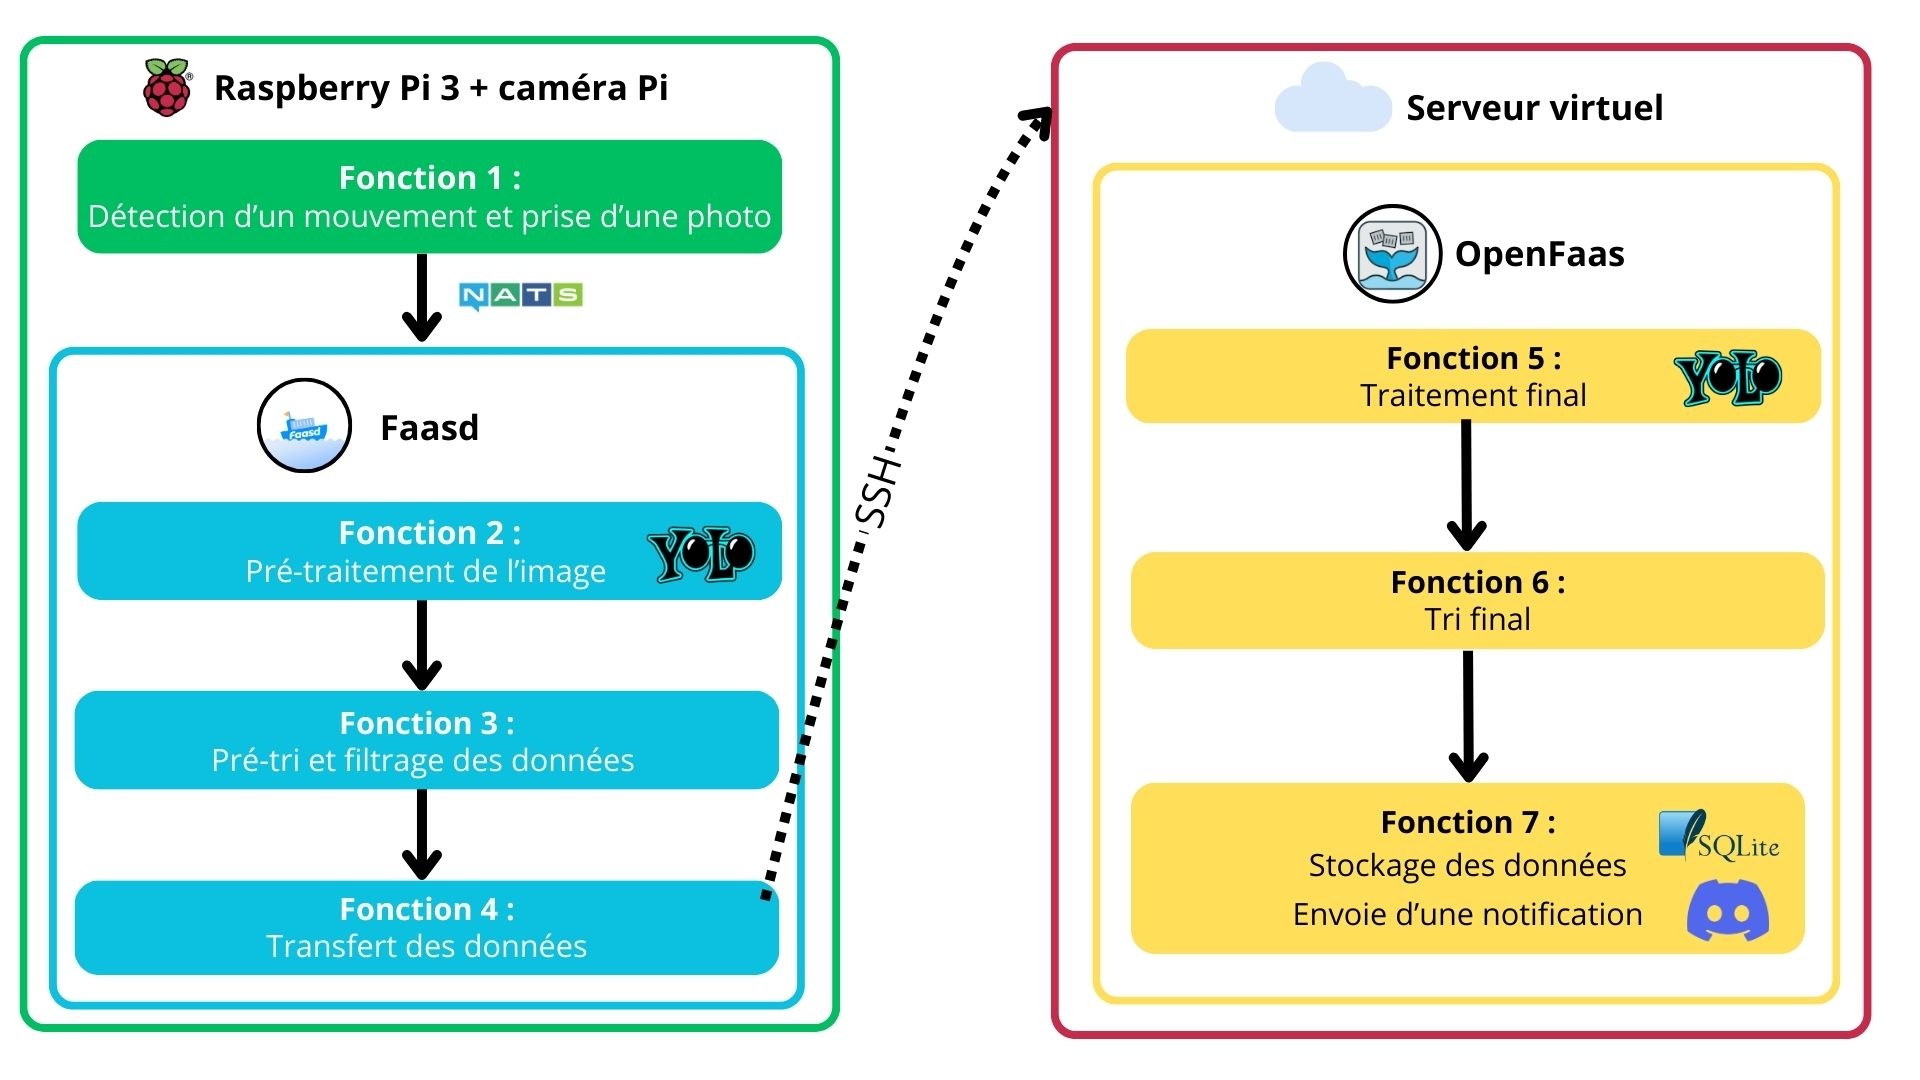
\includegraphics[scale=0.25]{architectureFinal.jpg}
		\caption{Architecture du projet}
		\label{fig1}
	\end{figure}
	
	\section{Base de données}
	
	\subsection{Technologie utilisée}
	\begin{itemize}
		\item SGBD : SQLite
		\item Deux tables principales :
		\begin{itemize}
			\item \textbf{Détections} : identifiant de la détection, classe détectée, nombre d'animaux de cette classe sur la photo, identifiant de la photo
			\item \textbf{Photos} : identifiant de la photo, heure, date, nombre total d'animaux sur la photo
		\end{itemize}
	\end{itemize}
	\begin{figure}[ht]
		\centering
		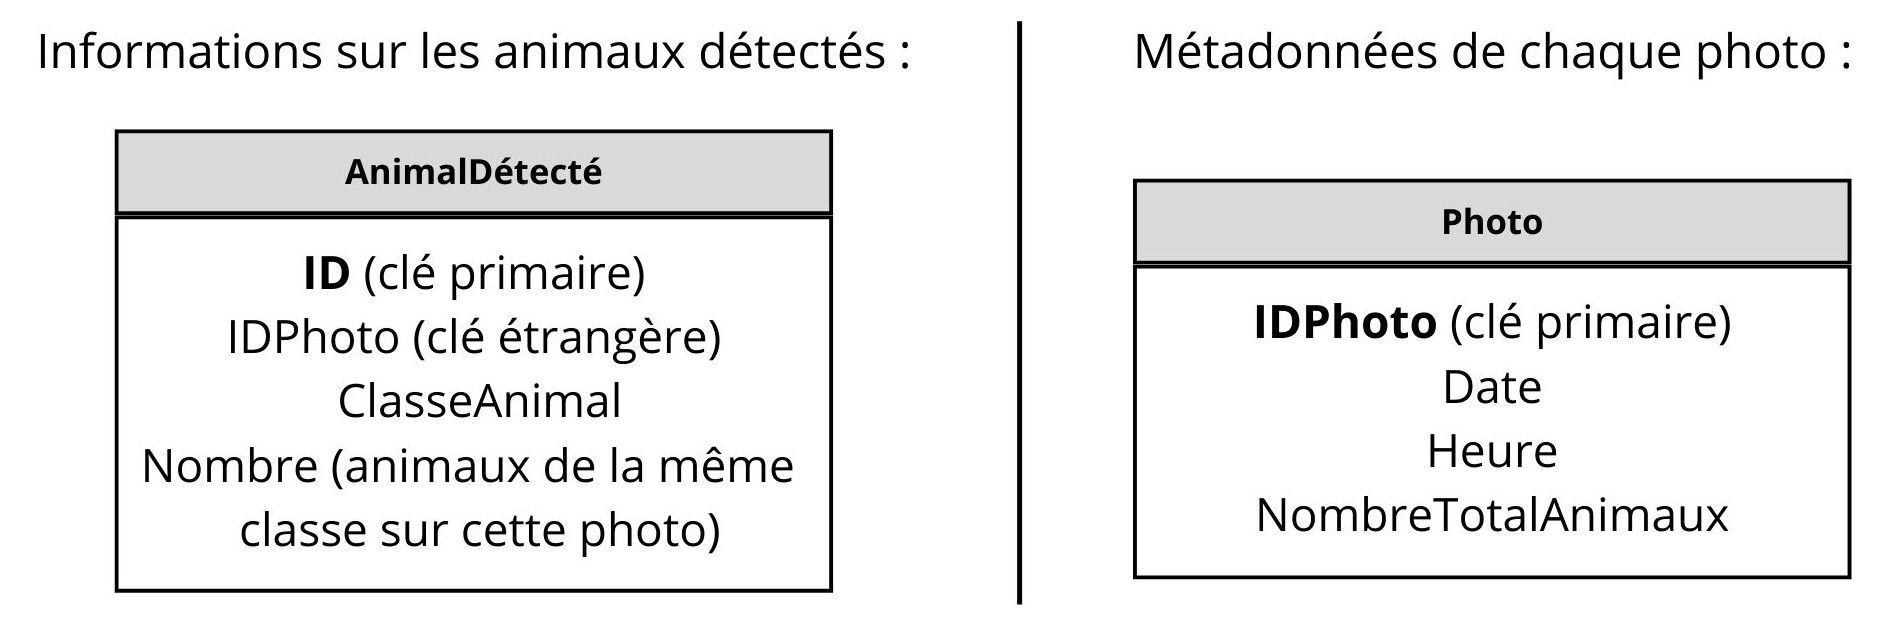
\includegraphics[scale=0.15]{BDD2.jpg}
		\caption{Tables de la base de données}
		\label{fig4}
	\end{figure}
	
	\subsection{Accès et exploitation}
	\begin{itemize}
		\item Requêtes simples via Python ou interface dédiée
		\item Ouverture de la base : \texttt{sqlite3 chemin/vers/taBase.db}
		\item Documentation SQLite : \texttt{.help}
		\item Sauvegarde avec : \texttt{sqlite3 database.db .dump}
		\item Fermeture de la base :  \texttt{.quit}\\
	\end{itemize}
	
	Pour plus de renseignements sur la formulations des requêtes SQLite : 
	\url{https://doc.ubuntu-fr.org/sqlite} 
	
	\section{Notification Discord}
	Afin d'envoyer un message sur un serveur discord, il est nécessaire de créer un bot. Voici les instructions pour le créer.\\\\
	\textbf{Etape 1 :} Activer le mode développeur dans les paramètres avancés de votre compte discord.\\
	\textbf{Etape 2 :}Dans le portail développeur, allez dans l'onglet "Application" et cliquez sur "Nouvelle application" puis donnez un nom à votre bot et copiez l'identifiant de l'application.\\
	\textbf{Etape 3 :} Dans l'onglet "Bot", cliquez sur "Ajouter un bot" afin de générer un compte bot ainsi qu'un jeton qui sera la clé d'accès du bot à Discord. \textbf{Attention :} ce jeton est à conserver en lieu sûr car sa divulgation pourrait exposer votre bot et votre serveur Discord à des risques de sécurité.\\
	\textbf{Etape 4 :}Dans l'onglet "Application", configurez les autorisations que vous accordez au bot.\\
	\textbf{Etape 5 :} Copiez l’URL générée en bas et ouvrez-la dans votre navigateur. Séléctionnez le bon serveur discord.\\
	\textbf{Etape 6 :} Installez la bibliothèque Discord.py : \texttt{pip install -U discord.py
	}\\
	\textbf{Etape 7:} Il ne reste plus qu'à écrire le code souhaiter en fonction des actions que vous désirez exécuter avec le bot. Il est important de placer le jeton du bot dans un fichier \texttt{.env} pour des raisons de sécurité.\\
	
	\begin{figure}[ht]
		\centering
		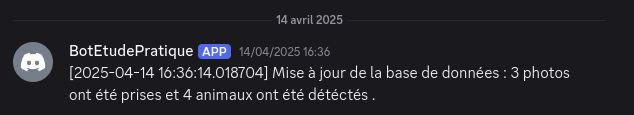
\includegraphics[scale=0.4]{Discord.png}
		\caption{Réception de la notification Discord}
		\label{fig5}
	\end{figure}
	
	\textbf{Documentation :}
	\begin{itemize}
		\item Documentation Discord développer : \url{https://discord.com/developers/docs/intro}
		\item Tutoriel configuration du bot : \url{https://www.ionos.fr/digitalguide/serveur/know-how/creer-un-bot-discord/}
		\item Documentation bibliothèque \texttt{discord.py}: \url{https://discordpy.readthedocs.io/en/stable/}
	\end{itemize}
	
	\section{Entraînement de YOLO}
		\textbf{Prérequis :} Un PC avec une carte graphique NVIDIA compatible CUDA ou utiliser Google Colab\\\\
		
		\textbf{Étape 1 : Installer Anaconda}
		\begin{itemize}
			\item Téléchargez l'installateur Anaconda pour votre système d'exploitation depuis : \url{https://www.anaconda.com/download}
			\item Lancez l'installateur et suivez les instructions 
			\item Une fois l'installation terminée, ouvrez le terminal Anaconda Prompt\\
		\end{itemize}
		
		\textbf{Étape 2 : Créer un environnement Python et installer Ultralytics}
		\begin{itemize}
			\item Dans le terminal Anaconda, créez un nouvel environnement Python : \texttt{conda create --name yolo8-env python=3.12 -y}
			\item Activez l'environnement : \texttt{conda activate yolo8-env}
			\item Installez la bibliothèque Ultralytics : \texttt{pip install ultralytics}
			\item Pour utiliser le GPU, installez la version correspondante de PyTorch (assurez-vous que votre GPU est compatible avec CUDA 12.4) : \texttt{pip install --upgrade torch torchvision torchaudio --index-url https://download.pytorch.org/whl/cu124}\\
		\end{itemize}
		
		\textbf{Étape 3 : Préparer les données}
		\begin{itemize}
			\item Collectez des images des objets que vous souhaitez détecter
			\item Utilisez l'outil d'annotation LabelImg pour étiqueter les objets dans les images : \url{https://github.com/tzutalin/labelImg}
			\item Organisez vos données dans une structure de dossiers conforme au format YOLO (dossier images, dossier labels et document classes.txt rassemblés dans un même dossier)
			\item Créez un fichier YAML (par exemple : data.yaml) décrivant votre jeu de données (path, train, val, nc, names)\\
		\end{itemize}
		
		\textbf{Étape 4 : Entraîner le modèle}\\
		Dans le terminal Anaconda, lancez l'entraînement avec la commande suivante (en adaptant les paramètres selon vos besoins) : \texttt{yolo task=detect mode=train model=yolov8n.pt data=data.yaml epochs=50 imgsz=640 batch=16 name=mon\_modele}\\
		
		\textbf{Étape 5 : Tester le modèle}\\
		Après l'entraînement, vous pouvez tester le modèle sur une image : \texttt{yolo task=detect mode=predict model=mon\_modele/weights/best.pt source=chemin/vers/image.jpg}\\

		\textbf{Documentation :}
		\begin{itemize}
			\item Tutoriel :  \url{https://www.ejtech.io/learn/train-yolo-models}
			\item Documentation Ultralytics : \url{https://docs.ultralytics.com/fr/modes/train/}\\
		\end{itemize}
	
	
	\section{Conclusion}
	Ce document présente l’environnement d’installation, l’architecture modulaire et le rôle de chaque fonction dans notre système. Le découplage local/cloud et l’approche \textit{serverless} ont permis de répondre aux contraintes matérielles tout en assurant extensibilité et efficacité.
	
	\vspace{1em}
	
\end{document}
